\documentclass[12pt,a4paper]{article}

% Margin: atas 3cm, bawah 3cm, kanan 3cm, kiri 4cm, kertas A4
\usepackage[top=3cm,bottom=3cm,right=3cm,left=4cm,a4paper]{geometry}

\usepackage{graphicx}
\usepackage{listings}
\usepackage{xcolor}
\usepackage[hidelinks]{hyperref}
\usepackage{fancyhdr}
\usepackage{setspace}
\usepackage{indentfirst}
\usepackage{amsmath}
\usepackage{float}
\usepackage{multirow}
\usepackage{ragged2e}
\usepackage{titlesec}
\usepackage{caption}
\usepackage[indonesian]{babel}
\usepackage[none]{hyphenat}
\usepackage{microtype}

\sloppy
\emergencystretch=2em

% Semua teks utama 12pt, spasi 1.15, rata kiri-kanan
\setstretch{1.15}
\AtBeginDocument{\justifying\normalsize}

% Paragraf
\setlength{\parindent}{1.25cm}
\setlength{\parskip}{0pt}

% Section dan subsection tetap 12pt, hanya bold
\titleformat{\section}
  {\normalfont\normalsize\bfseries}
  {\thesection}{1em}{}

\titleformat{\subsection}
  {\normalfont\normalsize\bfseries}
  {\thesubsection}{1em}{}

\titleformat{\subsubsection}
  {\normalfont\normalsize\bfseries}
  {\thesubsubsection}{1em}{}

% Caption gambar/tabel juga 12pt
\captionsetup{
    font=normalsize,
    labelfont=bf
}

% Nama daftar isi
\renewcommand{\contentsname}{Daftar Isi}

% rename figure to Gambar
\renewcommand{\figurename}{Gambar}

% Style untuk listing kode
\definecolor{codegreen}{rgb}{0,0.6,0}
\definecolor{codegray}{rgb}{0.5,0.5,0.5}
\definecolor{codepurple}{rgb}{0.58,0,0.82}
\definecolor{backcolour}{rgb}{0.95,0.95,0.92}

\lstdefinestyle{mystyle}{
    backgroundcolor=\color{backcolour},
    commentstyle=\color{codegreen},
    keywordstyle=\color{magenta},
    numberstyle=\tiny\color{codegray},
    stringstyle=\color{codepurple},
    basicstyle=\ttfamily\footnotesize,
    numbers=left,
    numbersep=5pt,
    breaklines=true,
    breakatwhitespace=false,
    columns=fullflexible,
    keepspaces=true,
    showspaces=false,
    showstringspaces=false,
    showtabs=false,
    tabsize=2,
    captionpos=b,
    postbreak=\mbox{\textcolor{codegray}{$\hookrightarrow$}\space}
}
\lstset{style=mystyle}

\begin{document}

% Halaman Cover
\begin{titlepage}
    \thispagestyle{empty}
    \centering
    \vspace*{-1.2cm}

    {\normalsize\bfseries Laporan Mini Project\par}
    \vspace{0.25cm}
    {\normalsize\bfseries Jam Digital 4-Digit dengan Fitur Dimming\par}

    \vspace{1.4cm}

    
\includegraphics[width=0.5\textwidth]{assets/img/logo-depart.png}

    \vspace{1.4cm}

    {\normalsize\bfseries Mata Kuliah\par}
    \vspace{0.2cm}
    {\normalsize Sistem Mikroprosesor dan Mikrokontroller\par}

    \vspace{0.8cm}

    {\normalsize\bfseries Dosen Pengampu\par}
    \vspace{0.2cm}
    {\normalsize Eko Pramunanto, S.T., M.T.\par}

    \vspace{1.1cm}

    {\normalsize\bfseries Disusun oleh\par}
    \vspace{0.25cm}
    {\normalsize Yuke Brilliant Hestiavin\par}
    {\normalsize 5024241016\par}

    \vfill

    {\normalsize\
    Departemen Teknik Komputer\\
    Fakultas Teknologi Elektro dan Informatika Cerdas\\
    Institut Teknologi Sepuluh Nopember\\
    Surabaya, 3 Juni 2026
    \par}
\end{titlepage}

\pagenumbering{roman}
\tableofcontents
\newpage

\pagenumbering{arabic}

\section{Pendahuluan}

\subsection{Latar Belakang}
Dalam pengembangan sistem embedded, kemampuan untuk menampilkan informasi waktu secara real-time dan menyesuaikan tampilan dengan kondisi lingkungan merupakan fitur yang sangat penting. Mini project ini bertujuan untuk mengimplementasikan jam digital menggunakan modul Real Time Clock (RTC) DS1307 dan tampilan 7-segment TM1637, serta menambahkan fitur pengaturan kecerahan atau dimming menggunakan potensiometer sebagai simulasi kontrol adaptif.

Melalui mini project ini, mahasiswa dapat memahami bagaimana mikrokontroler ESP32 membaca data waktu dari modul RTC, menampilkannya ke display 4 digit, serta membaca input analog dari potensiometer melalui ADC. Nilai analog tersebut kemudian digunakan untuk mengatur tingkat kecerahan display secara dinamis.

\subsection{Tujuan}
Tujuan dari mini project ini adalah sebagai berikut:
\begin{itemize}
    \item Memahami cara kerja dan komunikasi I2C pada modul RTC DS1307.
    \item Mengimplementasikan tampilan waktu menggunakan modul 4-digit 7-segment TM1637.
    \item Mempelajari konsep Analog to Digital Converter (ADC) pada ESP32 untuk membaca nilai potensiometer.
    \item Menerapkan teknik pemetaan nilai atau mapping untuk mengontrol kecerahan tampilan berdasarkan input analog.
    \item Mengimplementasikan sistem sederhana yang menggabungkan konsep mikrokontroler, sensor analog, dan aktuator tampilan digital.
\end{itemize}

\section{Dasar Teori}

\subsection{Real Time Clock (RTC) DS1307}
Real Time Clock atau RTC DS1307 adalah modul pewaktu yang dapat menyimpan dan menjaga informasi waktu secara real-time. Modul ini tetap dapat mempertahankan data waktu meskipun catu daya utama dimatikan karena dilengkapi dengan baterai cadangan.

RTC DS1307 berkomunikasi dengan mikrokontroler menggunakan protokol I2C atau Inter-Integrated Circuit. Komunikasi I2C hanya membutuhkan dua jalur utama, yaitu SDA sebagai jalur data dan SCL sebagai jalur clock. Pada ESP32, pin I2C yang umum digunakan adalah GPIO21 untuk SDA dan GPIO22 untuk SCL.

\subsection{Modul Tampilan TM1637}
TM1637 adalah modul driver display yang digunakan untuk mengontrol tampilan 7-segment 4 digit. Modul ini banyak digunakan pada proyek jam digital, stopwatch, counter, dan sistem tampilan angka sederhana lainnya.

Keunggulan modul TM1637 adalah jumlah pin yang dibutuhkan relatif sedikit, yaitu hanya dua pin kendali berupa CLK dan DIO. Selain itu, modul ini juga menyediakan fitur pengaturan kecerahan atau brightness yang dapat dikontrol melalui program.

\subsection{Analog to Digital Converter (ADC)}
Analog to Digital Converter atau ADC adalah fitur yang digunakan untuk mengubah sinyal analog menjadi nilai digital. Pada ESP32, ADC memiliki resolusi hingga 12-bit, sehingga nilai hasil pembacaan berada pada rentang 0 hingga 4095.

Pada mini project ini, ADC digunakan untuk membaca nilai tegangan dari potensiometer. Potensiometer bekerja sebagai pembagi tegangan, sehingga perubahan posisi putaran potensiometer menghasilkan perubahan tegangan pada pin ADC. Nilai ADC tersebut kemudian dipetakan ke rentang kecerahan TM1637, yaitu 0 hingga 7.

\subsection{Dimming}
Dimming adalah proses pengaturan tingkat kecerahan suatu tampilan atau lampu. Pada sistem ini, dimming diterapkan pada modul TM1637 dengan mengubah nilai brightness berdasarkan input dari potensiometer. Semakin besar nilai ADC yang terbaca, semakin tinggi tingkat kecerahan tampilan.

\section{Implementasi: Jam Digital 4-Digit dengan Fitur Dimming}

\subsection{Deskripsi}
Mini project ini membuat sebuah jam digital 4 digit yang menampilkan waktu berupa jam dan menit. Data waktu diperoleh dari modul RTC DS1307, kemudian ditampilkan pada modul 7-segment TM1637. Selain itu, sistem dilengkapi dengan potensiometer 10k$\Omega$ yang digunakan untuk mengatur tingkat kecerahan display.

ESP32 berperan sebagai mikrokontroler utama yang membaca data RTC, membaca nilai potensiometer melalui ADC, memproses nilai brightness, dan mengirimkan data waktu ke display TM1637.

\subsection{Komponen yang Digunakan}
Komponen yang digunakan pada mini project ini adalah sebagai berikut:
\begin{itemize}
    \item Mikrokontroler ESP32.
    \item Modul RTC DS1307.
    \item Modul tampilan 4-digit 7-segment TM1637.
    \item Potensiometer 10k$\Omega$.
    \item Kabel jumper.
    \item Breadboard.
\end{itemize}

\subsection{Rangkaian (Wiring Diagram)}
Rangkaian mini project ini menghubungkan ESP32 dengan modul RTC DS1307 melalui komunikasi I2C. Modul TM1637 dihubungkan ke dua pin digital ESP32, sedangkan potensiometer dihubungkan ke pin ADC untuk membaca nilai analog.

\begin{figure}[H]
    \centering
    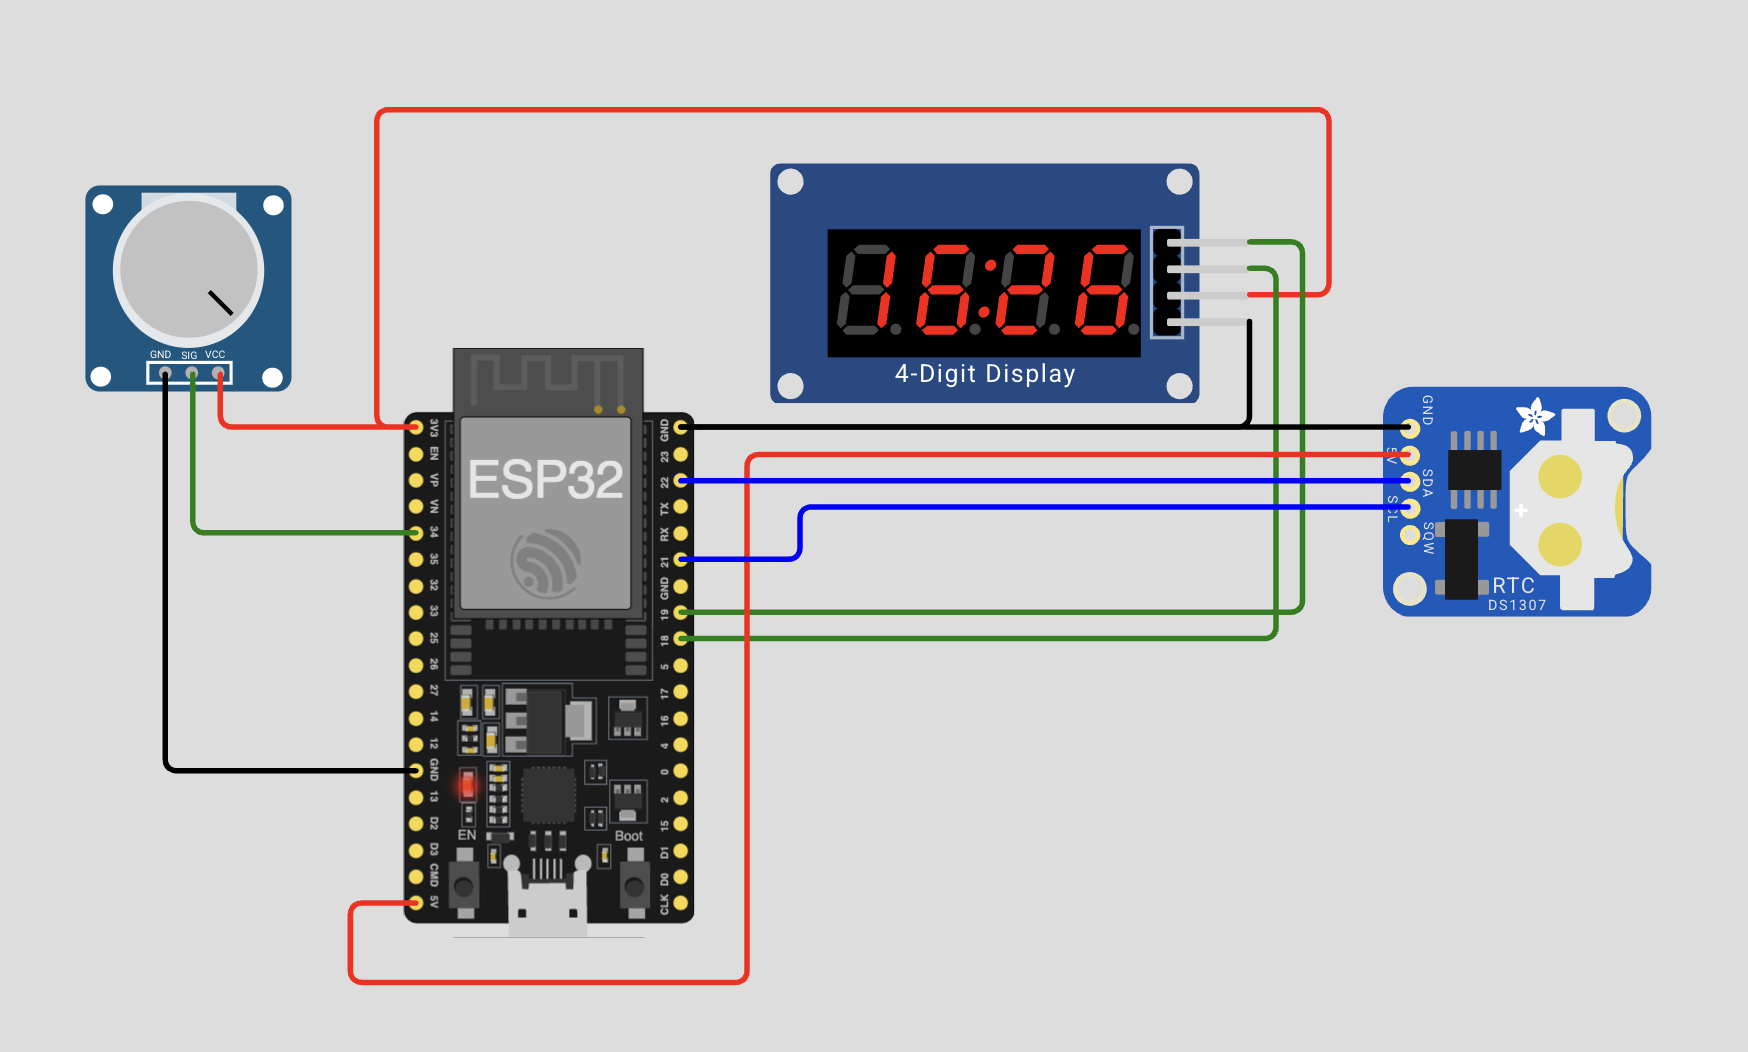
\includegraphics[width=0.82\textwidth]{assets/img/wiring-clock.png}
    \caption{Wiring diagram jam digital dengan RTC DS1307, TM1637, dan potensiometer}
    \label{fig:wiring-clock}
\end{figure}

Tabel \ref{tab:wiring-clock} berikut menjelaskan detail koneksi pin antara ESP32 dengan komponen-komponen pada rangkaian jam digital.

\begin{table}[H]
    \centering
    \caption{Detail Koneksi Pin Rangkaian Jam Digital}
    \label{tab:wiring-clock}
    \begin{tabular}{|l|l|l|l|}
        \hline
        \textbf{Komponen} & \textbf{Pin Komponen} & \textbf{Pin ESP32} & \textbf{Keterangan} \\
        \hline
        \multirow{4}{*}{RTC DS1307} & VCC & 5V & Catu daya modul \\
         & GND & GND & Ground \\
         & SDA & GPIO 21 & Data I2C \\
         & SCL & GPIO 22 & Clock I2C \\
        \hline
        \multirow{4}{*}{TM1637} & VCC & 5V & Catu daya display \\
         & GND & GND & Ground \\
         & CLK & GPIO 19 & Clock signal \\
         & DIO & GPIO 18 & Data I/O \\
        \hline
        \multirow{3}{*}{Potensiometer} & Kaki 1 & 3V3 & Referensi tegangan \\
         & Wiper (tengah) & GPIO 34 & Input ADC \\
         & Kaki 3 & GND & Ground \\
        \hline
    \end{tabular}
\end{table}

\subsection{Kode Program}
Kode program berikut digunakan untuk membaca waktu dari RTC DS1307, menampilkan waktu pada TM1637, dan mengatur tingkat kecerahan display berdasarkan nilai potensiometer.

\lstinputlisting[language=C++, caption={Kode program jam digital 4-digit dengan fitur dimming}]{assets/code/clock.cpp}

\subsection{Hasil dan Pembahasan}
Berdasarkan implementasi yang telah dilakukan, sistem berhasil menampilkan waktu real-time dari RTC DS1307 ke modul TM1637. Tampilan menunjukkan informasi jam dan menit dalam format 4 digit. Fitur titik dua atau colon pada display juga dapat dibuat berkedip sebagai indikator bahwa sistem berjalan secara normal.

Nilai analog dari potensiometer dibaca menggunakan fungsi \texttt{analogRead()} pada pin ADC ESP32. Nilai yang terbaca berada pada rentang 0 hingga 4095. Nilai tersebut kemudian dipetakan menggunakan fungsi \texttt{map()} ke rentang 0 hingga 7, sesuai dengan level brightness yang didukung oleh modul TM1637.

\begin{figure}[H]
    \centering
    \begin{minipage}{0.45\textwidth}
        \centering
        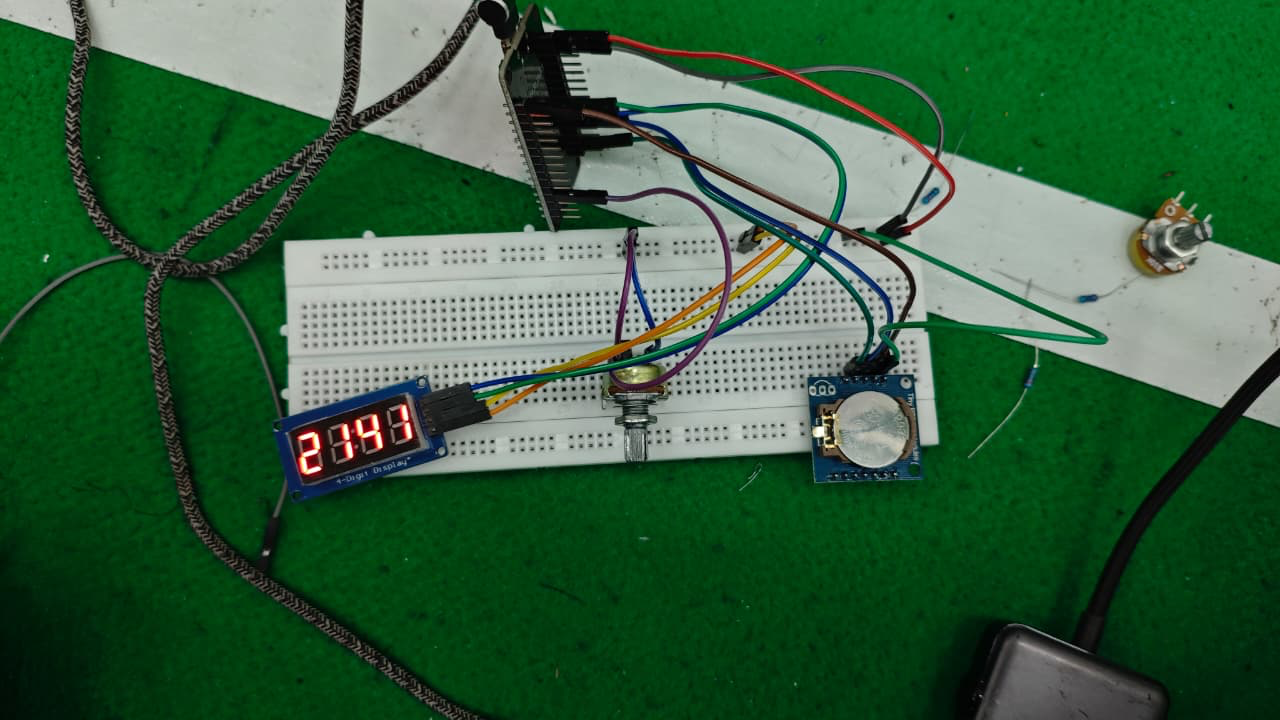
\includegraphics[width=\textwidth]{assets/img/clock-terang.png}
        \caption{Kondisi jam digital dengan kecerahan maksimal}
        \label{fig:clock-terang}
    \end{minipage}
    \hfill
    \begin{minipage}{0.45\textwidth}
        \centering
        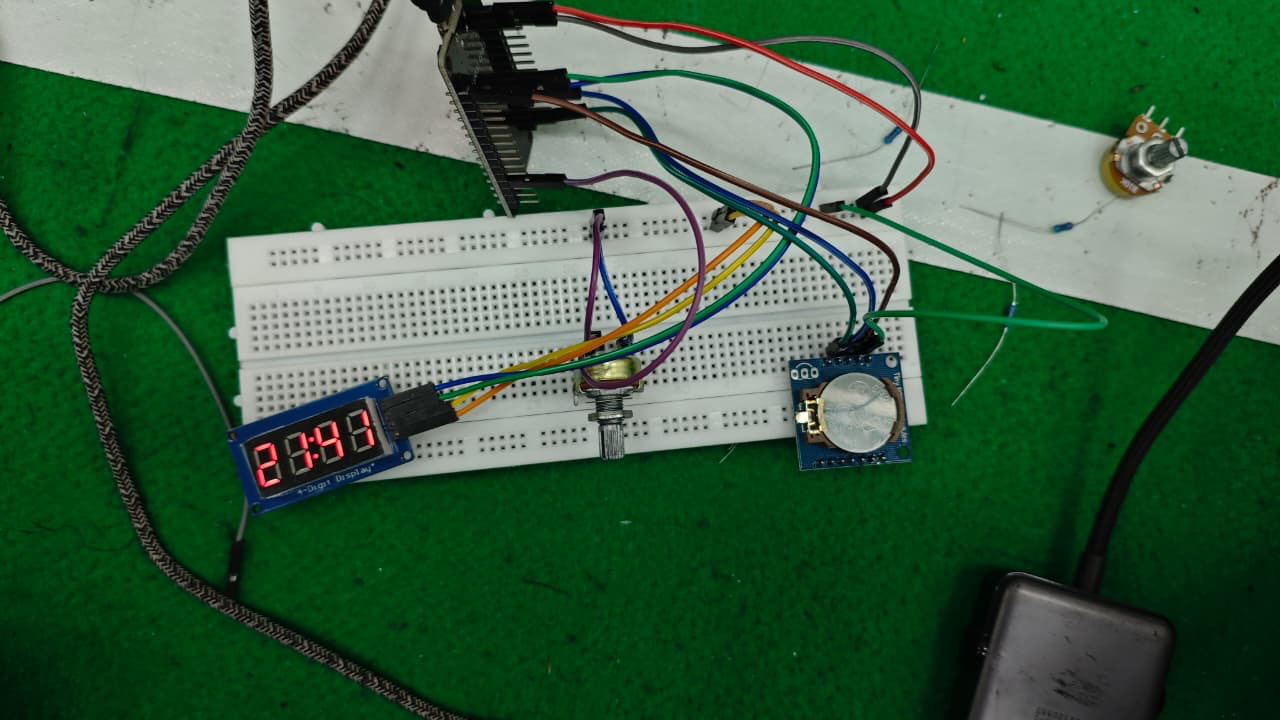
\includegraphics[width=\textwidth]{assets/img/clock-redup.png}
        \caption{Kondisi jam digital dengan kecerahan redup}
        \label{fig:clock-redup}
    \end{minipage}
\end{figure}

Pada Gambar \ref{fig:clock-terang} dan Gambar \ref{fig:clock-redup}, terlihat bahwa tingkat kecerahan display dapat berubah sesuai dengan putaran potensiometer. Ketika nilai potensiometer tinggi, display menyala lebih terang. Sebaliknya, ketika nilai potensiometer rendah, display menjadi lebih redup.

Fitur ini menunjukkan penerapan konsep ADC dan mapping nilai pada sistem mikrokontroler. Input analog dari potensiometer tidak langsung digunakan begitu saja, tetapi diproses terlebih dahulu agar sesuai dengan rentang nilai yang dibutuhkan oleh modul output.

\section{Kesimpulan}
Berdasarkan mini project yang telah dibuat, dapat disimpulkan bahwa:
\begin{enumerate}
    \item Modul RTC DS1307 berhasil berkomunikasi dengan ESP32 melalui protokol I2C untuk menyediakan data waktu secara real-time.
    \item Modul TM1637 dapat digunakan untuk menampilkan waktu dalam format 4 digit dengan penggunaan pin yang sederhana.
    \item ADC pada ESP32 dapat membaca nilai analog dari potensiometer dengan baik pada rentang 0 hingga 4095.
    \item Fungsi \texttt{map()} efektif digunakan untuk mengubah rentang nilai ADC menjadi rentang kecerahan TM1637, yaitu 0 hingga 7.
    \item Mini project ini berhasil menggabungkan konsep RTC, display digital, ADC, dan dimming dalam satu sistem embedded sederhana.
\end{enumerate}

\end{document}